\subsubsection{Optimizer: Optimization Passes on Parsed IR}

Usually there are two kinds of compiler Optimization (Opt) passes, one is analysis passes and the other is transform passes.
Currently our analysis pass is mainly Dominator Tree analysis pass,
while transform passes contains Dead Code Elimination (DCE), Promote Memory to Register (Mem2Reg), Sparse Conditional Constant Propagation (SCCP).

Its pipeline process is as \figref{fig:ola-lang-backend-ir-opt}:
\begin{figure}[!htbp]
    \centering
    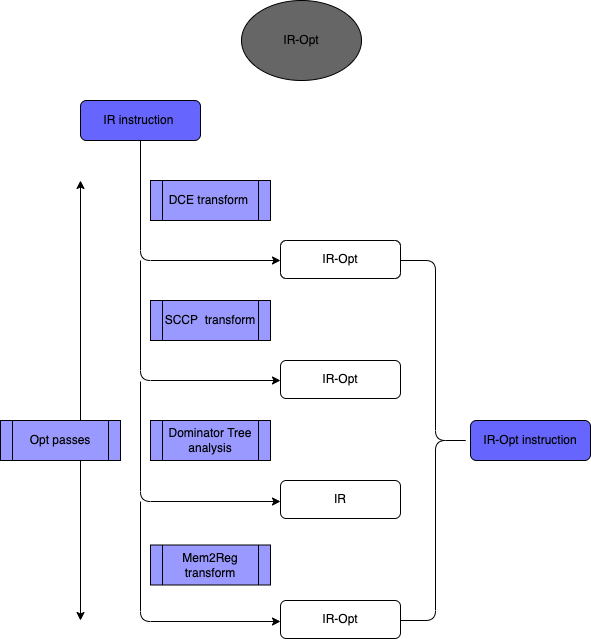
\includegraphics[width=0.6\textwidth]{ola-lang-backend-ir-opt.png}
    \caption{Ola-lang Backend IR Optimization}
    \label{fig:ola-lang-backend-ir-opt}
\end{figure}
